\section{Deriving a pure functional approach}
\label{sec:functional_approach}

We presented a high-level agent-based approach to the SIR model in the previous section, which focused only on the states and the transitions, but we haven't talked about technical implementation.

In \cite{thaler_art_2017} two fundamental problems of implementing an agent-based simulation from a programming-language agnostic point of view is discussed. The first problem is how agents can be pro-active and the second how interactions and communication between agents can happen. For agents to be pro-active, they must be able to perceive the passing of time, which means there must be a concept of an agent-process which executes over time. Interactions between agents can be reduced to the problem of how an agent can expose information about its internal state which can be perceived by other agents.

In this section we will derive a pure functional approach for an agent-based simulation of the SIR model in which we will pose solutions to the previously mentioned problems. We will start out with a very naive approach and show its limitations which we overcome by adding FRP. Then in further steps we will add more concepts and generalisations, ending up at the final approach which utilises monadic stream functions (MSF), a generalisation of FRP 
\footnote{The code of all steps can be accessed freely through the following URL: \url{https://github.com/thalerjonathan/phd/tree/master/public/purefunctionalepidemics/code}}.

\subsection{Naive beginnings}
\label{sec:naive_beginnigs}
We start by modelling the states of the agents:

\begin{HaskellCode}
data SIRState = Susceptible | Infected TimeDelta | Recovered
\end{HaskellCode}

Agents are ill for some duration, meaning we need to keep track when a potentially infected agent recovers. Also a simulation is stepped in discrete or continuous time-steps thus we introduce a notion of \textit{time} and $\Delta t$ by defining:

\begin{HaskellCode}
type Time      = Double
type TimeDelta = Double
\end{HaskellCode}

Now we can represent every agent simply as the SIR state which includes its potential recovery time. We hold all our agents in a list:
\begin{HaskellCode}
type SIRAgent = SIRState
type Agents   = [SIRAgent]
\end{HaskellCode}

Next we need to think about how to actually step our simulation. For this we define a function which advances our simulation with a fixed $\Delta t$ until a given time $t$ where in each step the agents are processed and the output is fed back into the next step. This is the source of pro-activity as agents are executed in every time step and can thus initiate actions based on the passing of time.
As already mentioned, the agent-based implementation of the SIR model is inherently stochastic which means we need access to a random-number generator. We decided to use the Random Monad at this point as threading a generator through the simulation and the agents could become very cumbersome. Thus our simulation stepping runs in the Random Monad:
TODO: make clear we are stepping by a dt of 1.0 which is necessary below

\begin{HaskellCode}
runSimulation :: RandomGen g 
  => Time -> Agents -> Rand g [Agents]
runSimulation tEnd as = runSimulationAux 0 as []
  where
    runSimulationAux :: RandomGen g 
      => Time -> Agents -> [Agents] -> Rand g [Agents]
    runSimulationAux t as acc
      | t >= tEnd = return (reverse (as : acc))
      | otherwise = do
        as' <- stepSimulation as 
        runSimulationAux (t + 1.0) as' (as : acc)

stepSimulation :: RandomGen g => Agents -> Rand g Agents
stepSimulation as = mapM (runAgent as) as
\end{HaskellCode}

Now we can implement the behaviour of an individual agent. First we need to distinguish between the agents SIR states:

\begin{HaskellCode}
processAgent :: RandomGen g 
  => Agents -> SIRAgent -> Rand g SIRAgent
processAgent as Susceptible    = susceptibleAgent as
processAgent _  (Infected dur) = return (infectedAgent dur)
processAgent _  Recovered      = return Recovered
\end{HaskellCode}

An agent gets fed the states of all agents in the system from the previous time-step so it can draw random contacts - this is one, very naive way of implementing the interactions between agents.

From our implementation it becomes apparent that only the behaviour of a susceptible agent involves randomness and that a recovered agent is simply a sink - it does nothing and stays constant.

Lets look how we can implement the behaviour of a susceptible agent. It simply makes contact on average with a number of other agents and gets infected with a given probability if an agent it has contact with is infected.
When the agent gets infected, it calculates also its time of recovery by drawing a random number from the exponential distribution, meaning it is ill on average for \textit{illnessDuration}.
TODO: make clear that this only works for dt=1.0, if we change dt then we would need to adjust contact rate (multiply) but the discretisation using floor will lead to wrong results

\begin{HaskellCode}
susceptibleAgent :: RandomGen g => Agents -> Rand g SIRAgent
susceptibleAgent as = do
    -- draws from exponential distribution
    rc <- randomExpM (1 / contactRate) 
    cs <- replicateM (floor rc) (makeContact as)
    if or cs
      then infect
      else return Susceptible
  where
    makeContact :: RandomGen g => Agents -> Rand g Bool
    makeContact as = do
      randContact <- randomElem as
      case randContact of
        -- returns True with given probability 
        (Infected _) -> randomBoolM infectivity 
        _            -> return False

    infect :: RandomGen g => Rand g SIRAgent
    infect = randomExpM (1 / illnessDuration) 
               >>= \rd -> return (Infected rd)
\end{HaskellCode}

The infected agent is trivial. It simply recovers after the given illness duration which is implemented as follows:
TODO: explain that we are using fixed dt=1.0

\begin{HaskellCode}
infectedAgent :: TimeDelta -> TimeDelta -> SIRAgent
infectedAgent dur
    | dur' <= 0 = Recovered
    | otherwise = Infected dur'
  where
    dur' = dur - 1.0  
\end{HaskellCode}

\subsubsection{Results}
When running our naive implementation with a population size of 1,000 we get the dynamics as seen in Figure \ref{fig:sir_abs_dynamics_naive}. When comparing it to the dynamics of the analytical solution in Figure \ref{fig:sir_sd_dynamics}, the agent-based dynamics are not as smooth which stems from the fact that the agent-based approach is inherently discrete and stochastic \cite{macal_agent-based_2010}. Also we are using a $\Delta t = 1.0$ which means that we are under-sampling the contact-rate. We will will address this problem in the next section.

\begin{figure}
	\centering
	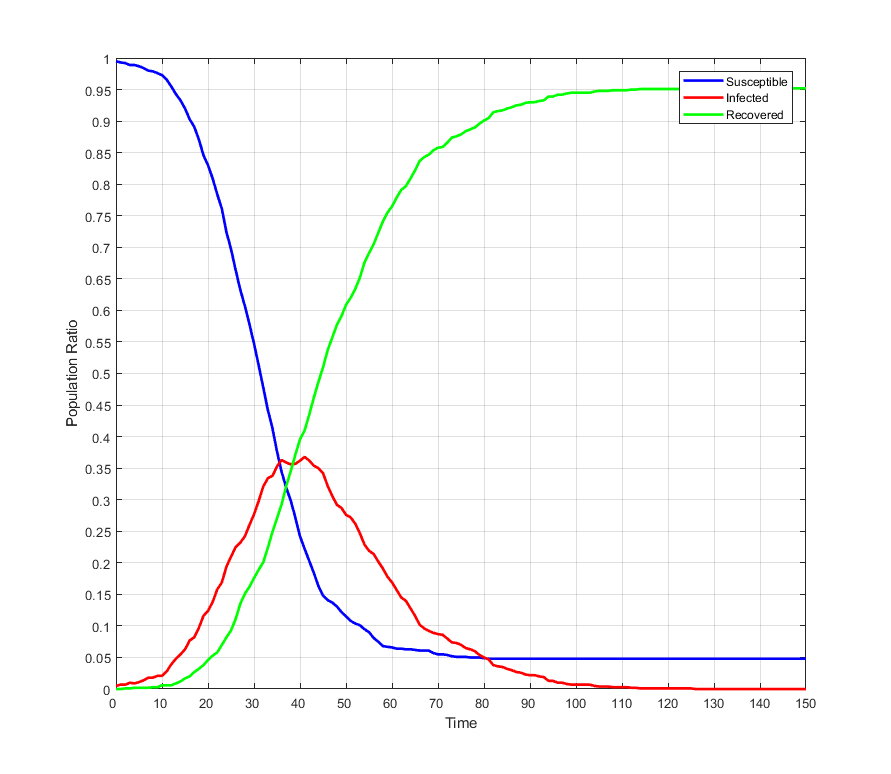
\includegraphics[width=0.35\textwidth, angle=0]{./fig/step1_randmonad/SIR_1000agents_150t_1dt.png}
	\caption{Naive simulation of SIR using the agent-based approach. Population of 1,000, contact rate $\beta = \frac{1}{5}$, infection probability $\gamma = 0.05$, illness duration $\delta = 15$ with initially 1 infected agent. Simulation run for 150 time-steps with fixed $\Delta t = 1.0$.}
	\label{fig:sir_abs_dynamics_naive}
\end{figure}

%\begin{figure}
%\begin{center}
%	\begin{tabular}{c}
%		\begin{subfigure}[b]{0.2\textwidth}
%			\centering
%			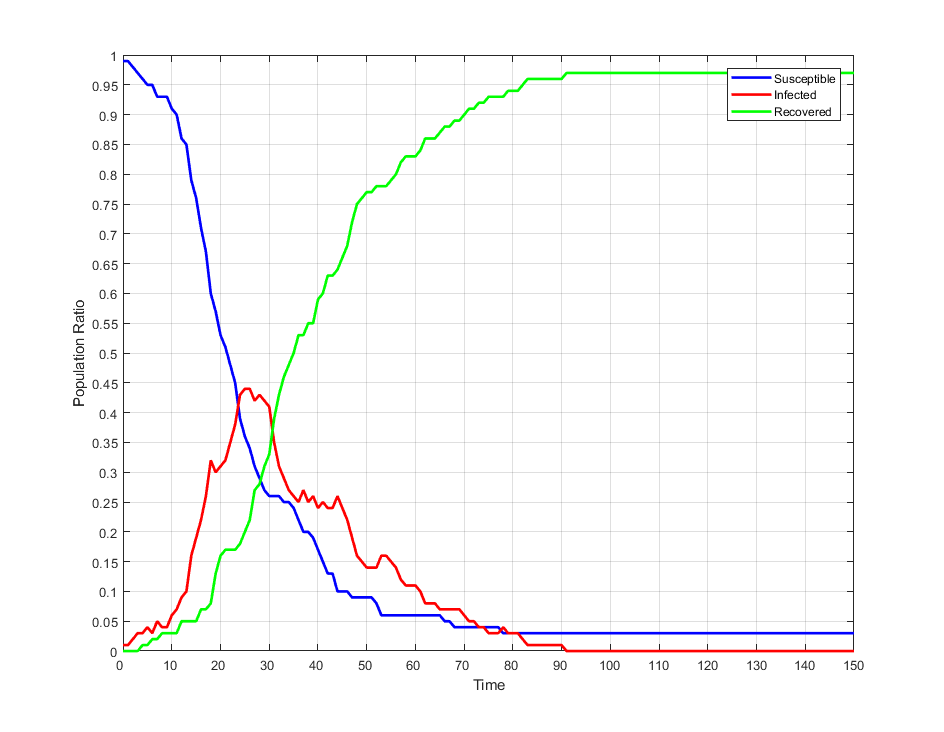
\includegraphics[width=1.0\textwidth, angle=0]{./fig/step1_randmonad/SIR_100agents_150t_1dt.png}
%			\caption{100 Agents}
%			\label{fig:sir_abs_approximating_1dt_100agents}
%		\end{subfigure}
    	
%    	&
%    	
%		\begin{subfigure}[b]{0.30\textwidth}
%			\centering
%			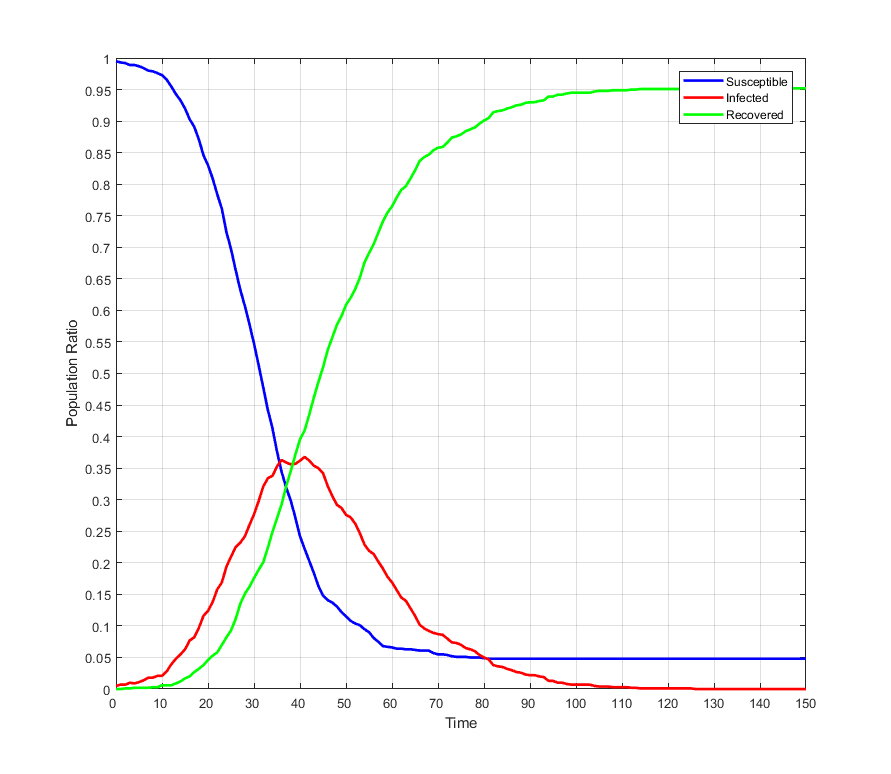
\includegraphics[width=1.0\textwidth, angle=0]{./fig/step1_randmonad/SIR_1000agents_150t_1dt.png}
%			\caption{1,000 Agents}
%			\label{fig:sir_abs_approximating_1dt_1000agents}
%		\end{subfigure}
%	\end{tabular}
%	\caption{TODO: use only 1000, a simulation with 100 has slightly different dynamics in SD as well! Naive simulation of SIR using the agent-based approach. Varying population size, contact rate $\beta = \frac{1}{5}$, infection probability $\gamma = 0.05$, illness duration $\delta = 15$ with initially 1 infected agent. Simulation run for 150 time-steps with fixed $\Delta t = 1.0$.} 
%	\label{fig:sir_abs_dynamics_naive}
%\end{center}
%\end{figure}

\subsubsection{Discussion}
Reflecting on our first naive approach we can conclude that it already introduced most of the fundamental concepts of ABS
\begin{itemize}
	\item Time - the simulation occurs over virtual time which is modelled explicitly divided into \textit{fixed} $\Delta t$ where at each step all agents are executed.
	\item Agents - we implement each agent as an individual, with the behaviour depending on its state.
	\item Feedback - the output state of the agent in the current time-step $t$ is the input state for the next time-step $t + \Delta t$.
	\item Environment - as environment we implicitly assume a fully-connected network (complete graph) where every agent 'knows' every other agent, including itself and thus can make contact with all of them.
	\item Stochasticity - it is an inherently stochastic simulation, which is indicated by the Random Monad type and the usage of \textit{randomBoolM} and \textit{randomExpM}.
	\item Deterministic - repeated runs with the same initial random-number generator result in same dynamics. This may not come as a surprise but in Haskell we can guarantee that property statically already at compile time because our simulation runs in the Random Monad and \textit{not} in the IO Monad. This guarantees that no external, uncontrollable sources of randomness can interfere with the simulation.
	\item Dynamics - with increasing number of agents the dynamics smooth out \cite{macal_agent-based_2010}.
\end{itemize}

TODO: problem is that we implicitly assume that TimeDelta is always 1.0, still it is not ensured in all agents

Nonetheless our approach has also weaknesses and dangers:
\begin{enumerate}
	\item We are implicitly assuming that our implementation is sampling with 1.0
	\item $\Delta t$ is passed explicitly as argument to the agent and needs to be dealt with explicitly. This is not very elegant and a potential source of errors - can we do better and find a more elegant solution? 
	\item The way our agents are represented is not very modular. The state of the agent is explicitly encoded in an ADT and when processing the agent, the behavioural function always needs to distinguish between the states. Can we express it in a more modular way e.g. continuations?
\end{enumerate}

We now move on to the next section in which we will address these points and the under-sampling issue.

\subsection{Functional Reactive Programming}
\label{sec:step2_frp}
As described in the Section \ref{sec:back_frp}, Arrowized FRP \cite{hughes_generalising_2000} is a way to implement systems  with continuous and discrete time-semantics where the central concept is the Signal Function, which can be understood as a process over time, mapping an input- to an output-signal. Technically speaking, a signal function is a continuation which allows to capture state using closures and hides away the $\Delta t$ which means that it is never exposed explicitly to the programmer, meaning it cannot be messed with.

The concept of processes over time is an ideal match for our agents and our system as a whole thus we will implement them and the whole system as signal functions.

\subsubsection{Implementation}
We start by defining the SIR states as ADTs and our agents as signal function (SF) which receives the SIR states of all agents as input and outputs the current SIR state of the agent:

\begin{HaskellCode}
data SIRState = Susceptible | Infected | Recovered

type SIRAgent = SF [SIRState] SIRState 
\end{HaskellCode}

Now we can define the behaviour of an agent to be the following:

\begin{HaskellCode}
sirAgent :: RandomGen g => g -> SIRState -> SIRAgent
sirAgent g Susceptible = susceptibleAgent g
sirAgent g Infected    = infectedAgent g
sirAgent _ Recovered   = recoveredAgent
\end{HaskellCode}

Depending on the initial state we return the corresponding behaviour. Note that we are passing a random-number generator instead of running in the Random Monad because signal functions as implemented in Yampa are not capable of being monadic. 

We see that the recovered agent ignores the random-number generator because a recovered agent does nothing, stays immune forever and can not get infected again in this model. Thus a recovered agent is a consuming state from which there is no escape, it simply acts as a sink which returns constantly \textit{Recovered}:

\begin{HaskellCode}
recoveredAgent :: SIRAgent
recoveredAgent = arr (const Recovered)
\end{HaskellCode}

Lets look how we can implement the behaviour of a susceptible agent. It makes contact \textit{on average} with $\beta$ other random agents. For every \textit{infected} agent it gets into contact with, it becomes infected with a probability of $\gamma$. If an infection happens, it makes the transition to the \textit{Infected} state. To make contact, it gets fed the states of all agents in the system from the previous time-step so it can draw random contacts - this is one, very naive way of implementing the interactions between agents.

Thus a susceptible agent behaves as susceptible until it becomes infected. Upon infection an \textit{Event} is returned which results in switching into the \textit{infectedAgent} SF, which causes the agent to behave as an infected agent from that moment on. When an infection event occurs we change the behaviour of an agent using the Yampa combinator \textit{switch}, which is quite elegant and expressive as it makes the change of behaviour at the occurrence of an event explicit. Note that to make contact \textit{on average}, we use Yampas \textit{occasionally} function which requires us to carefully select the right $\Delta t$ for sampling the system as will be shown in results. 

%\begin{samepage}
\begin{HaskellCode}
susceptibleAgent :: RandomGen g => g -> SIRAgent
susceptibleAgent g = 
    switch (susceptible g) (const (infectedAgent g))
  where
    susceptible :: RandomGen g 
      => g -> SF [SIRState] (SIRState, Event ())
    susceptible g = proc as -> do
      makeContact <- occasionally g (1 / contactRate) () -< ()
      if isEvent makeContact
        then (do
          -- draw random element from the list
          a <- drawRandomElemSF g -< as
          case a of
            Infected -> do
              -- returns True with given probability
              i <- randomBoolSF g infectivity -< ()
              if i
                then returnA -< (Infected, Event ())
                else returnA -< (Susceptible, NoEvent)
             _       -> returnA -< (Susceptible, NoEvent))
        else returnA -< (Susceptible, NoEvent)
\end{HaskellCode}
%\end{samepage}

To deal with randomness in an FRP way we implemented additional signal functions built on the \textit{noiseR} function provided by Yampa. This is an example for the stream character and statefulness of a signal function as it allows to keep track of the changed random-number generator internally through the use of continuations and closures. Here we provide the implementation of \textit{randomBoolSF}. \textit{drawRandomElemSF} works similar but takes a list as input and returns a randomly chosen element from it:

\begin{HaskellCode}
randomBoolSF :: RandomGen g => g -> Double -> SF () Bool
randomBoolSF g p = proc _ -> do
  r <- noiseR ((0, 1) :: (Double, Double)) g -< ()
  returnA -< (r <= p)
\end{HaskellCode}

An infected agent recovers \textit{on average} after $\delta$ time units. This is implemented by drawing the duration from an exponential distribution \cite{borshchev_system_2004} with $\lambda = \frac{1}{\delta}$ and making the transition to the \textit{Recovered} state after this duration. Thus the infected agent behaves as infected until it recovers, on average after the illness duration, after which it behaves as a recovered agent by switching into \textit{recoveredAgent}. As in the case of the susceptible agent, we use the \textit{occasionally} function to generate the event when the agent recovers. Note that the infected agent ignores the states of the other agents as its behaviour is completely independent of them.

\begin{HaskellCode}
infectedAgent :: RandomGen g => g -> SIRAgent
infectedAgent g = switch infected (const recoveredAgent)
  where
    infected :: SF [SIRState] (SIRState, Event ())
    infected = proc _ -> do
      recEvt <- occasionally g illnessDuration () -< ()
      let a = event Infected (const Recovered) recEvt
      returnA -< (a, recEvt)
\end{HaskellCode}

For running the simulation we use Yampas function \textit{embed}:

\begin{HaskellCode}
runSimulation :: RandomGen g 
  => g -> Time -> DTime -> [SIRState] -> [[SIRState]]
runSimulation g t dt as 
    = embed (stepSimulation sfs as) ((), dts)
  where
    steps     = floor (t / dt)
    dts       = replicate steps (dt, Nothing)
    n         = length as
    (rngs, _) = rngSplits g n [] -- unique rngs for each agent
    sfs       = zipWith sirAgent rngs as
\end{HaskellCode}

What we need to implement next is a closed feedback-loop - the heart of every agent-based simulation. Fortunately, \cite{nilsson_functional_2002, courtney_yampa_2003} discusses implementing this in Yampa. The function \textit{stepSimulation} is an implementation of such a closed feedback-loop. It takes the current signal functions and states of all agents, runs them all in parallel and returns this step's new agent states. Note the use of \textit{notYet} which is required because in Yampa switching occurs immediately at $t = 0$. If we don't delay the switching at $t = 0$ until the next step, we would enter an infinite switching loop - \textit{notYet} simply delays the first switching until the next time-step.

\begin{HaskellCode}
stepSimulation :: [SIRAgent] -> [SIRState] -> SF () [SIRState]
stepSimulation sfs as =
    dpSwitch
      -- feeding the agent states to each SF
      (\_ sfs' -> (map (\sf -> (as, sf)) sfs'))
      -- the signal functions
      sfs
      -- switching event, ignored at t = 0         
      (switchingEvt >>> notYet)
      -- recursively switch back into stepSimulation         
      stepSimulation                            
  where
    switchingEvt :: SF ((), [SIRState]) (Event [SIRState])
    switchingEvt = arr (\ (_, newAs) -> Event newAs)
\end{HaskellCode}

Yampa provides the \textit{dpSwitch} combinator for running signal functions in parallel, which has the following type-signature:

\begin{HaskellCode}
dpSwitch :: Functor col
         -- routing function
         => (forall sf. a -> col sf -> col (b, sf))
         -- SF collection
         -> col (SF b c)
         -- SF generating switching event     
         -> SF (a, col c) (Event d)
         -- continuation to invoke upon event           
         -> (col (SF b c) -> d -> SF a (col c))
         -> SF a (col c)
\end{HaskellCode}

Its first argument is the pairing-function which pairs up the input to the signal functions - it has to preserve the structure of the signal function collection. The second argument is the collection of signal functions to run. The third argument is a signal function generating the switching event. The last argument is a function which generates the continuation after the switching event has occurred. \textit{dpSwitch} returns a new signal function which runs all the signal functions in parallel and switches into the continuation when the switching event occurs. The d in \textit{dpSwitch} stands for decoupled which guarantees that it delays the switching until the next time-step: the function into which we switch is only applied in the next step, which prevents an infinite loop if we switch into a recursive continuation.

Conceptually, \textit{dpSwitch} allows us to recursively switch back into the \textit{stepSimulation} with the continuations and new states of all the agents after they were run in parallel. 

\subsubsection{Results}
The dynamics generated by this step can be seen in Figure \ref{fig:sir_abs_dynamics_frp}. 

\begin{figure}
\begin{center}
	\begin{tabular}{c c}
		\begin{subfigure}[b]{0.22\textwidth}
			\centering
			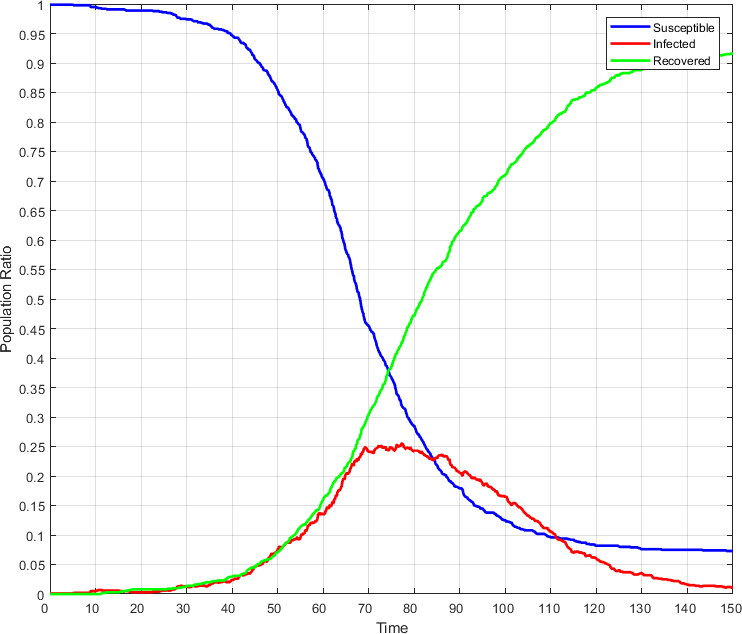
\includegraphics[width=1\textwidth, angle=0]{./fig/step2_yampa/SIR_1000agents_150t_01dt.png}
			\caption{$\Delta t = 0.1$}
			\label{fig:sir_abs_approximating_01dt_1000agents}
		\end{subfigure}
		
		&
    	
		\begin{subfigure}[b]{0.22\textwidth}
			\centering
			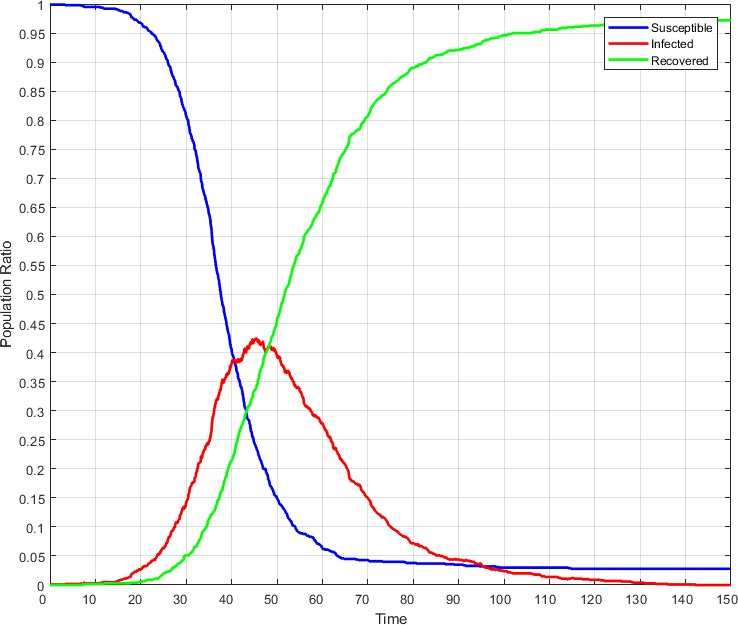
\includegraphics[width=1\textwidth, angle=0]{./fig/step2_yampa/SIR_1000agents_150t_001dt.png}
			\caption{$\Delta t = 0.01$}
			\label{fig:sir_abs_approximating_001dt_1000agents}
		\end{subfigure}
	\end{tabular}
	
	\caption{FRP simulation of agent-based SIR showing the influence of different $\Delta t$. Population size of 1,000 with contact rate $\beta = \frac{1}{5}$, infection probability $\gamma = 0.05$, illness duration $\delta = 15$ with initially 1 infected agent. Simulation run for 150 time-steps with respective $\Delta t$.} 
	\label{fig:sir_abs_dynamics_frp}
\end{center}
\end{figure}

By following the FRP approach we assume a continuous flow of time which means that we need to select a \textit{correct} $\Delta t$ otherwise we would end up with wrong dynamics. The selection of a correct $\Delta t$ depends in our case on \textit{occasionally} in the \textit{susceptible} behaviour, which randomly generates an event on average with \textit{contact rate} following the exponential distribution. To arrive at the correct dynamics, this requires us to sample \textit{occasionally}, and thus the whole system, with small enough $\Delta t$ which matches the frequency of events generated by \textit{contact rate}. If we choose a too large $\Delta t$, we loose events which will result in wrong dynamics as can be seen in Figure \ref{fig:sir_abs_approximating_01dt_1000agents}. This issue is known as under-sampling and is described in Figure \ref{fig:sampling_issue}.

\begin{figure}
\begin{center}
	\begin{tabular}{c}
		\begin{subfigure}[b]{0.3\textwidth}
			\centering
			
\includegraphics[width=1\textwidth, angle=0]{./fig/diagrams/Undersampling.png}
			\caption{Under-sampling}
			\label{fig:undersampling}
		\end{subfigure}
		
		\\
		
		\begin{subfigure}[b]{0.3\textwidth}
			\centering
			
\includegraphics[width=1\textwidth, angle=0]{./fig/diagrams/Supersampling.png}
			\caption{Super-sampling}
			\label{fig:supersampling}
		\end{subfigure}
	\end{tabular}
	
	\caption{A visual explanation of under-sampling and super-sampling. The black dots represent the time-steps of the simulation. The red dots represent virtual events which occur at specific points in continuous time. In the case of under-sampling, 3 events occur in between the two time steps but \textit{occasionally} only captures the first one. By increasing the sampling frequency either through a smaller $\Delta t$ or super-sampling all 3 events can be captured.} 
	\label{fig:sampling_issue}
\end{center}
\end{figure}

For tackling this issue we have two options. The first one is to use a smaller $\Delta t$ as can be seen \ref{fig:sir_abs_approximating_001dt_1000agents}, which results in the whole system being sampled more often, thus reducing performance. The other option is to implement super-sampling and apply it to \textit{occasionally} which would allow us to run the whole simulation with $\Delta t = 1.0$ and only sample the \textit{occasionally} function with a much higher frequency.

An approach to super-sampling would be to introduce a new combinator to Yampa which allows us to super-sample other signal functions. 

\begin{HaskellCode}
superSampling :: Int -> SF a b -> SF a [b]
\end{HaskellCode}

It evaluates the \textit{SF} argument for \textit{n} times, each with $\Delta t = \frac{\Delta t}{n}$ and the same input argument \textit{a} for all \textit{n} evaluations. At time 0 no super-sampling is performed and just a single output of the \textit{SF} argument is calculated. A list of \textit{b} is returned with length of \textit{n} containing the result of the \textit{n} evaluations of the \textit{SF} argument. If 0 or less super samples are requested exactly one is calculated. We could then wrap the occasionally function which would then generate a list of events. We have investigated super-sampling more in-depth but have to omit this due to lack of space.

\subsubsection{Discussion}
We can conclude that our first step already introduced most of the fundamental concepts of ABS:
\begin{itemize}
	\item Time - the simulation occurs over virtual time which is modelled explicitly divided into \textit{fixed} $\Delta t$ where at each step all agents are executed.
	\item Agents - we implement each agent as an individual, with the behaviour depending on its state.
	\item Feedback - the output state of the agent in the current time-step $t$ is the input state for the next time-step $t + \Delta t$.
	\item Environment - as environment we implicitly assume a fully-connected network (complete graph) where every agent 'knows' every other agent, including itself and thus can make contact with all of them.
	\item Stochasticity - it is an inherently stochastic simulation, which is indicated by the random-number generator and the usage of \textit{occasionally}, \textit{randomBoolSF} and \textit{drawRandomElemSF}.
	\item Deterministic - repeated runs with the same initial random-number generator result in same dynamics. This may not come as a surprise but in Haskell we can guarantee that property statically already at compile time because our simulation runs \textit{not} in the IO Monad. This guarantees that no external, uncontrollable sources of non-determinism can interfere with the simulation.
\end{itemize}

Using FRP in the instance of Yampa results in clarity, expressivity and robustness of our implementation. State is implicitly encoded, depending on which signal function is active. By using explicit time-semantics with \textit{occasionally} we can achieve extremely fine grained stochastics by sampling the system with small $\Delta t$: we are treating it as a truly continuous time-driven agent-based system.

A very severe problem, very hard to find with testing but detectable with in-depth validation analysis, is the fact that in the \textit{susceptible} agent the same random-number generator is used in \textit{occasionally}, \textit{drawRandomElemSF} and \textit{randomBoolSF}. This means that all three stochastic functions, which should be independent from each other, are inherently correlated. This is something one wants to prevent under all circumstances in a simulation, as it can invalidate the dynamics on a very subtle level, and indeed we have tested the influence of the correlation in this example and it has an impact. We left this severe bug in for explanatory reasons, as it shows an example where functional programming actually encourages very subtle bugs if one is not careful. A possible solution would be to simply split the initial random-number generator in \textit{sirAgent} three times (using one of the splited generators for the next split) and pass three random-number generators to \textit{susceptible}.

So far we have an acceptable implementation of an agent-based SIR approach. What we are lacking at the moment is a general treatment of an environment. To conveniently introduce it we want to make use of monads which is not possible using Yampa. In the next step we make the transition to Monadic Stream Functions as introduced in Dunai \cite{perez_functional_2016} which allows FRP within a monadic context.

\subsection{Generalising to Monadic Stream Functions}
\label{sec:generalising_msfs}
A part of the library Dunai is BearRiver, a wrapper which re-implements Yampa on top of Dunai, which should allow us to easily replace Yampa with MSFs. This will enable us to run arbitrary monadic computations in a signal function, solving our problem of correlated random numbers through the use of the Random Monad.

\subsubsection{Identity Monad}
We start by making the transition to BearRiver by simply replacing Yampas signal function by BearRivers', which is the same but takes an additional type parameter \textit{m}, indicating the monadic context. If we replace this type-parameter with the Identity Monad, we should be able to keep the code exactly the same, because BearRiver re-implements all necessary functions we are using from Yampa. We simply re-define the agent signal function, introducing the monad stack our SIR implementation runs in:

\begin{HaskellCode}
type SIRMonad = Identity
type SIRAgent = SF SIRMonad [SIRState] SIRState
\end{HaskellCode}

\subsubsection{Random Monad}
Using the Identity Monad does not gain us anything but it is a first step towards a more general solution. Our next step is to replace the Identity Monad by the Random Monad, which will allow us to run the whole simulation within the Random Monad with the full features of FRP, finally solving the problem of correlated random numbers in an elegant way. We start by re-defining the SIRMonad and SIRAgent:

\begin{HaskellCode}
type SIRMonad g = Rand g
type SIRAgent g = SF (SIRMonad g) [SIRState] SIRState
\end{HaskellCode}

The question is now how to access this Random Monad functionality within the MSF context. For the function \textit{occasionally}, there exists a monadic pendant \textit{occasionallyM} which requires a MonadRandom type-class. Because we are now running within a MonadRandom instance we simply replace \textit{occasionally} with \textit{occasionallyM}. 

\begin{HaskellCode}
occasionallyM :: MonadRandom m => Time -> b -> SF m a (Event b)
-- can be used through the use of arrM and lift
randomBoolM :: RandomGen g => Double -> Rand g Bool
-- this can be used directly as a SF with the arrow notation
drawRandomElemSF :: MonadRandom m => SF m [a] a
\end{HaskellCode}

\subsubsection{Discussion} 
Running in the Random Monad solved the problem of correlated random numbers and elegantly guarantees us that we won't have correlated stochastics as discussed in the previous section. In the next step we introduce the concept of an explicit discrete 2D environment.

\subsection{Adding an environment}
\label{sec:adding_env}
So far we have implicitly assumed a fully connected network amongst agents, where each agent can see and 'knows' every other agent. This is a valid environment and in accordance with the System Dynamics inspired implementation of the SIR model but does not show the real advantage of ABS to situate agents within arbitrary environments. Often, agents are situated within a discrete 2D environment \cite{epstein_growing_1996} which is simply a finite $N x M$ grid with either a Moore or von Neumann neighbourhood (Figure \ref{fig:abs_neighbourhoods}). Agents are either static or can move freely around with cells allowing either single or multiple occupants.

We can directly map the SIR model to a discrete 2D environment by placing the agents on a corresponding 2D grid with an unrestricted neighbourhood. The behaviour of the agents is the same but they select their interactions directly from the shared read-only environment, which will be passed to the agents as input. This allows agents to read the states of all their neighbours which tells them if a neighbour is infected or not. To show the benefit over the System Dynamics approach  and for purposes of a more interesting approach, we restrict the neighbourhood to Moore (Figure \ref{fig:moore_neighbourhood}).

\begin{figure}
\begin{center}
	\begin{tabular}{c c}
		\begin{subfigure}[b]{0.2\textwidth}
			\centering
			
\includegraphics[width=0.5\textwidth, angle=0]{./fig/diagrams/neumann.png}
			\caption{von Neumann}
			\label{fig:neumann_neighbourhood}
		\end{subfigure}
    	&
		\begin{subfigure}[b]{0.2\textwidth}
			\centering
			
\includegraphics[width=0.5\textwidth, angle=0]{./fig/diagrams/moore.png}
			\caption{Moore}
			\label{fig:moore_neighbourhood}
		\end{subfigure}
    \end{tabular}
	\caption{Common neighbourhoods in discrete 2D environments of Agent-Based Simulation.}
	\label{fig:abs_neighbourhoods}
\end{center}
\end{figure}

We also implemented this spatial approach in Java using the well known ABS library RePast \cite{north_complex_2013}, to have a comparison with a state of the art approach and came to the same results as shown in Figure \ref{fig:sir_dunai}. This supports, that our pure functional approach can produce such results as well and compares positively to the state of the art in the ABS field.

\subsubsection{Implementation}
We start by defining the discrete 2D environment for which we use an indexed two dimensional array. Each cell stores the agent state of the last time-step, thus we use the \textit{SIRState} as type for our array data. Also, we re-define the agent signal function to take the structured environment \textit{SIREnv} as input instead of the list of all agents as in our previous approach. As output we keep the \textit{SIRState}, which is the state the agent is currently in. Also we run in the Random Monad as introduced before to avoid the random number correlation. 

\begin{HaskellCode}
type Disc2dCoord = (Int, Int)
type SIREnv      = Array Disc2dCoord SIRState

type SIRAgent g  = SF (Rand g) SIREnv SIRState
\end{HaskellCode}

Note that the environment is not returned as output because the agents do not directly manipulate the environment but only read from it. Again, this enforces the semantics of the \textit{parallel} update-strategy through the types where the agents can only see the previous state of the environment and see the actions of other agents reflected in the environment only in the next step.

Note that we could have chosen to use a StateT transformer with the \textit{SIREnv} as state, instead of passing it as input, with the agents then able to arbitrarily read/write, but this would have violated the semantics of our model because actions of agents would have become visible within the same time-step.

The implementation of the susceptible, infected and recovered agents are almost the same with only the neighbour querying now slightly different. 

Stepping the simulation needs a new approach because in each step we need to collect the agent outputs and update the environment for the next next step. For this we implemented a separate MSF, which receives the coordinates for every agent to be able to update the state in the environment after the agent was run. Note that we need use \textit{mapM} to run the agents because we are running now in the context of the Random Monad. This has the consequence that the agents are in fact run sequentially one after the other but because they cannot see the other agents actions nor observe changes in the shared read-only environment, it is \textit{conceptually} a \textit{parallel} update-strategy where agents run in lock-step, isolated from each other at conceptually the same time.
  
\begin{HaskellCode}
simulationStep :: RandomGen g => [(SIRAgent g, Disc2dCoord)]
               -> SIREnv -> SF (Rand g) () SIREnv
simulationStep sfsCoords env = MSF (\_ -> do
  let (sfs, coords) = unzip sfsCoords 
  -- run agents sequentially but with shared, read-only environment
  ret <- mapM (`unMSF` env) sfs
  -- construct new environment from all agent outputs for next step
  let (as, sfs') = unzip ret
      env' = foldr (\ (a, coord) envAcc -> updateCell coord a envAcc) 
               env (zip as coords)

      sfsCoords' = zip sfs' coords
      cont       = simulationStep sfsCoords' env'
  return (env', cont))
 
updateCell :: Disc2dCoord -> SIRState -> SIREnv -> SIREnv
\end{HaskellCode}

\subsubsection{Results}
We implemented rendering of the environments using the gloss library which allows us to cycle arbitrarily through the steps and inspect the spreading of the disease over time visually as seen in Figure \ref{fig:sir_dunai}.

\begin{figure}
\begin{center}
	\begin{tabular}{c c}
		\begin{subfigure}[b]{0.2\textwidth}
			\centering
			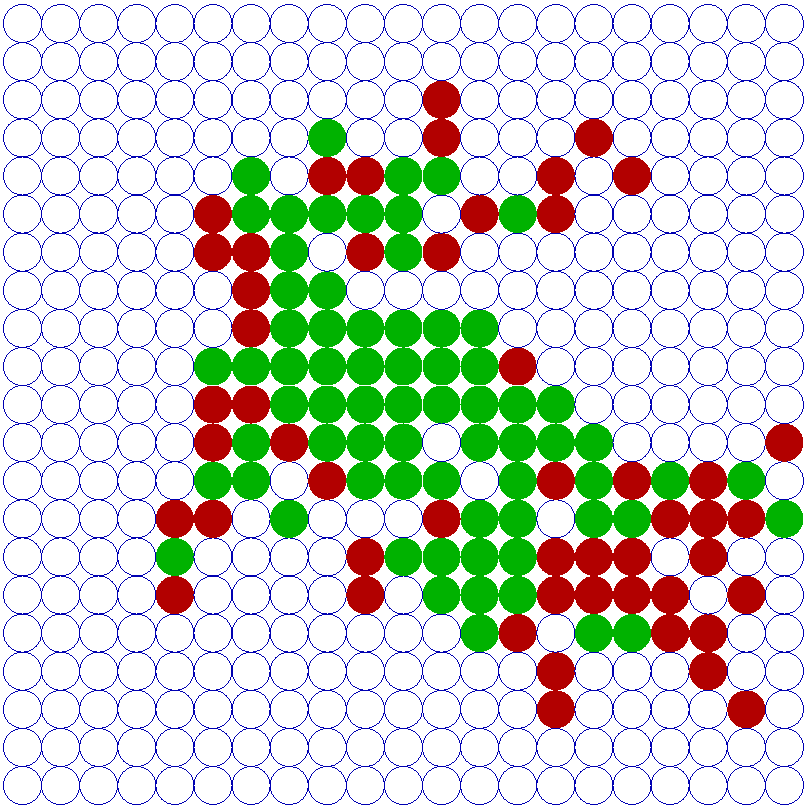
\includegraphics[width=1\textwidth, angle=0]{./fig/SIR_Dunai/SIR_Dunai_dt001_environment.png}
			\caption{Environment at $t = 50$}
			\label{fig:sir_dunai_env}
		\end{subfigure}
    	
    	&
  
		\begin{subfigure}[b]{0.23\textwidth}
			\centering
			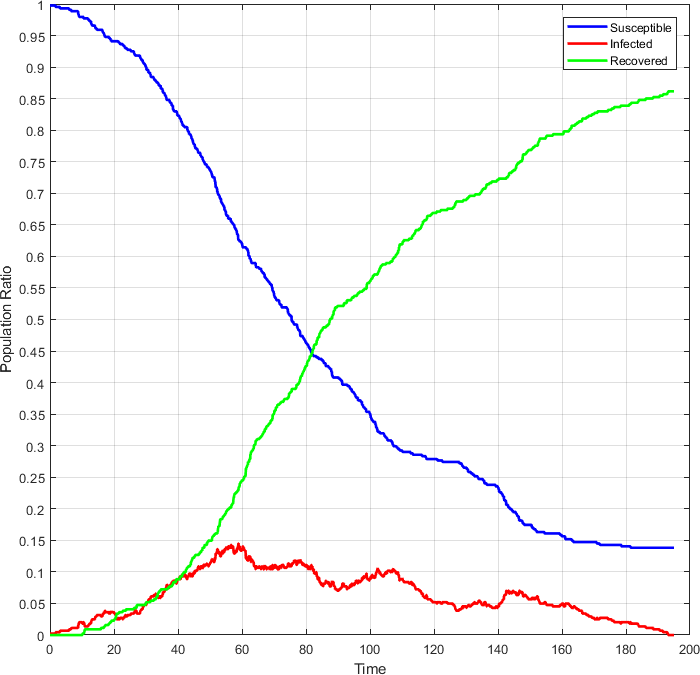
\includegraphics[width=1\textwidth, angle=0]{./fig/SIR_Dunai/SIR_Dunai_dt001.png}
			\caption{Dynamics over time}
			\label{fig:sir_dunai_env_dynamics}
		\end{subfigure}
	\end{tabular}
	
	\caption{Simulating the agent-based SIR model on a 21x21 2D grid with Moore neighbourhood (Figure \ref{fig:moore_neighbourhood}), a single infected agent at the center and same SIR parameters as in Figure \ref{fig:sir_sd_dynamics}. Simulation run until $t = 200$ with fixed $\Delta t = 0.01$. Last infected agent recovers around $t = 194$. The susceptible agents are rendered as blue hollow circles for better contrast.}
	\label{fig:sir_dunai}
\end{center}
\end{figure}

Note that the dynamics of the spatial SIR simulation which are seen in Figure \ref{fig:sir_dunai_env_dynamics} look quite different from the reference dynamics of Figure \ref{fig:sir_sd_dynamics}. This is due to a much more restricted neighbourhood which results in far fewer infected agents at a time and a lower number of recovered agents at the end of the epidemic, meaning that fewer agents got infected overall.

\subsubsection{Discussion}
By introducing a structured environment with a Moore neighbourhood, we showed the ABS ability to place the heterogeneous agents in a generic environment, which is the fundamental advantage of an agent-based approach over other simulation methodologies and allows us to simulate much more realistic scenarios.

Note, that an environment is not restricted to be a discrete 2D grid and can be anything from a continuous N-dimensional space to a complex network - one only needs to change the type of the environment and agent input and provide corresponding neighbourhood querying functions. 